% =====================================================================
%  Supplementary Materials -- Scientific Reports submission
%  Standalone, compiles with pdflatex.  Contains the complete audit
%  trail for the condensed main text; every number in the main text can
%  be traced to a note below.  No new data, numbers or claims are
%  introduced here: this file only carries material moved out of the
%  main text verbatim.
% =====================================================================
\documentclass[11pt,a4paper]{article}

\usepackage[utf8]{inputenc}
\usepackage[T1]{fontenc}
\usepackage{lmodern}
\usepackage[a4paper,margin=2.2cm]{geometry}
\usepackage{graphicx}
\usepackage{amsmath,amssymb}
\usepackage{booktabs}
\usepackage{array}
\usepackage{textcomp}
\usepackage[hidelinks]{hyperref}

\setlength{\parskip}{3pt}
\setlength{\parindent}{0pt}
\renewcommand{\arraystretch}{1.12}
\renewcommand{\thefigure}{S\arabic{figure}}

\title{\bfseries Supplementary Materials\\
\large Validation-first measurement of resilience in illicit data economies}
\author{Ziying Xue, Yongjin Chen, Songze Zhu}
\date{}

\begin{document}
\maketitle

\noindent\textbf{The Supplementary Materials contain the complete audit trail;
every number in the main text can be traced to a note below.} No number, claim
or citation is introduced here that is not already in the main text or in the
source analysis records.

\section*{S1. Complete protocol detail}

\subsection*{S1.1 The two-list rule}

When an instrument self-reports failure, the failure report itself is that
gate's output and must be given: how many cells fell outside the window, which
cells they were, what the window was, and the verbatim text of the decision
rule. What is forbidden is any quantity \emph{read off} the failed instrument ---
a point estimate, a band, a comparison, a significance statement. The test for
which list a reading belongs to is whether it can stand without the failed
instrument: cell identities and the window cannot, and are therefore reportable;
a shuffled-control AUC can, and is therefore withheld.

\subsection*{S1.2 What would falsify the protocol}

A protocol that cannot fail is not one. Three observations would count against
it, and each is checkable. (i) If, in a new domain, the G2 controls pass for
\emph{nearly every} candidate instrument, then G2 has no discriminating power
there and the gate is a formality. (ii) If the metrics G1 screens out bear no
relation to the metrics practitioners in that domain consider valid, G1 is
pedantry rather than protection. (iii) If the audit trail never changes a
reported number, and no quantity is ever withheld, downgraded or reversed by the
controls it is paired with, then G3 is bookkeeping. Our own corpus is a partial
answer in the opposite direction: the controls reversed four of our claims,
three instruments failed outright, and no metric cleared all three validity
gates, so the gates bit on this domain.

\subsection*{S1.3 The audit census}

The manifest has a time point and a domain, and both matter. Its domain is the
result artifacts this study produced; its time point is the manifest's build,
and artifacts produced after it are not in it. The artifacts counted are
\textbf{302 in all}, distributed across the top-level tree (196), the figures
subtree (25), and eight further subtree groups (40, 14, 9, 5, 5, 3, 3 and 2).
Earlier drafts reported \textbf{283} entries and flagged six de-leakage
artifacts carried outside them; that gap is closed here rather than carried
forward, and no artifact in the manifest's scope is unregistered. A later build
of the same tree added the eight outputs of the four pre-registered L4 cells ---
one JSON and one plain-text result file per cell --- and the totals above are
those of that build. Because a census is only as good as the rule that draws its
boundary, that rule --- which trees are walked and what counts as an artifact ---
is reproduced with the manifest, so that the count can be recomputed rather than
taken on trust.

\subsection*{S1.4 Reproduction discipline}

Cross-artifact agreement is required before a quantity may anchor an analysis:
two pipelines independently reproduced an address count of \textbf{61,487}. CPU
and GPU replicates are never tabulated together; on one replicate the largest
per-cell absolute difference in reported AUC was max $|d|$ = 0.0068 (cell 5/Q4),
against a pre-registered tolerance of 1e-3. Device-equivalence checks under fp64
deterministic mode reproduce bitwise across devices; fp32 forward passes exhibit
chaos amplification and are excluded from equivalence gates.

\section*{S2. Full controls, rejected estimators, specification curve and
metric validity}

\subsection*{S2.1 Full controls and every rejected estimator}

Every control reported in the main text, with the estimator it rejected, is
listed in the analysis table of the main text. Three entries carry additional
detail. For E7-inf, a second apparent effect (significant survival differences
across groups) reduces to a label-semantics difference between untagged
placeholder and source-probe groups and is disclosed as such; and one control is
vacuous by construction, since hosts carrying a single URL cannot produce a later
addition and both kinds read exactly 0.00\% against approximately 8\% floors.
For E0, the concentration proposition fails under clustered standard errors
(\textbf{p = 0.1736} by reporter, \textbf{p = 0.5978} by block) after the IID
standard error understated the block-clustered one by \textbf{14.44$\times$}. For
E5-fin, every p-value is withheld: between-step differences span $-27.4$ pp to
$+13.1$ pp, roughly 100$\times$ the nominal standard error, so the fixed-effect
standard error assumes a homogeneity the data violates.

\subsection*{S2.2 Specification curve (E1-v3)}

The demoted estimate's specification curve spans twelve core specifications that
vary the fixed-effect structure, the binning, the event definition, the target
market and the pre/post window. All twelve are estimable, every one is positive
and clears zero at the 5\% level, $\beta$ spans \textbf{3.2892 to 4.1176} with
median \textbf{3.7755}, and the positive share is \textbf{1.0}. The curve is
anchored to the incumbent analysis rather than standing free: with the candidate
set held equal it reproduces that analysis's coefficient exactly
($|\Delta\beta|$ = \textbf{0.00e+00}), and on its own candidate set the gap is
$|\Delta\beta|$ = \textbf{0.0360} (\textbf{3.6005} against \textbf{3.6365}) over
\textbf{489} candidates of which \textbf{158} are exposed. The five auxiliary
specifications span \textbf{2.2926 to 4.2076}, and one of them does not clear
zero (\textbf{0.1468}, p = 0.2723). The corrected magnitudes, \textbf{+1.0424}
and \textbf{+2.4426}, come from designs whose nulls sit near zero and lie below
this range rather than inside it. The curve varies the specification, not the
placebo machinery, so it does not re-test the parallel-trends violation, and its
breadth is not an interval estimate.

\subsection*{S2.3 Exploratory cross-layer association (WP4)}

Thirteen usable months; the association between the social layer's monthly
feedback volume and the financial layer's monthly transaction volume is read as
a lag profile over lags $-3$ to $+3$. The same-period association is
\textbf{r = -0.7206}, the largest absolute correlation in the window, with the
next-largest at lag $+1$ ($|r|$ = 0.6867). The circular-shift null (10,000 draws)
degenerates on a window-maximum statistic: the profile maximum is deterministic
under shift, so the draws take only \textbf{4 distinct values} and \textbf{50.4\%}
of them fall on the observed value itself; the 95\% interval collapses to
\textbf{[0.5365, 0.7206]} and the in-artifact \textbf{p = 0.5038} is a tautology
rather than a test. We therefore claim nothing about whether the layers are
coupled. This analysis is exploratory and is not one of the seven controlled
analyses.

\subsection*{S2.4 Metric-validity matrix}

Six candidate resilience metrics were screened against three pre-registered
criteria: rank recovery against a planted truth without collapsing onto another
metric's truth, calibration whose slope interval covers 1 and intercept interval
covers 0, and separation from a week-permuted null. \textbf{Each criterion passes
two of the six metrics, and no metric passes all three}; two metrics pass two of
the three. The metric with the highest own-truth correlation
(\texttt{recovery\_time}, Spearman \textbf{0.9859}) fails the rank criterion
because it is indistinguishable from \texttt{centrality\_redistribution} (max
$|$cross-Spearman$|$ = \textbf{0.8407} $\geq$ 0.8), and the two metrics that pass
the rank criterion fail the permutation criterion by construction. The artifact
lists the three criteria without stating a conjunction rule, so any single count
of survivors is a post-hoc choice; we report the per-criterion matrix. The six
metric \emph{names} come from the pre-registered plan while their operational
definitions are ours, so none of this validates the delivered E1 measure.

\section*{S3. Per-configuration anatomy of the negative results}

\subsection*{S3.1 De-leakage configurations (E5p/E5r)}

Read on the within-entry-step metric the arms are judged on: configuration L1
keeps nine of the as-built arm's ten features (all but the calendar column) and
reads \textbf{0.7155632}, \emph{above} the as-built baseline of
\textbf{0.7136417}; configuration L2 keeps three features and reads
\textbf{0.6560979}; configuration L3 reads exactly \textbf{0.5000} and the
artifact marks it at chance, but L3 retains only the stratifying variable itself,
and a single feature constant within every bin yields an AUC of exactly one half
by construction, so L3 is a vacuous control and its 0.5 is not evidence of
repair. \textbf{The strongest non-vacuous configuration moves the control from
0.7136 to 0.6561 and stops there.} The values 0.633 / 0.652 / 0.681 that the
same artifact reports are its \emph{pooled} per-horizon figures, which the
artifact itself notes are not comparable to 0.5. One limitation is declared
inside the artifact: the de-leakage removes node and tabular feature columns,
but graph message passing still runs over the full snapshot graph. An untrained
model of the same architecture already separates at up to \textbf{0.6378}
(GraphSAGE, $\Delta = 1$), and across the three configurations the untrained
GraphSAGE readings span \textbf{0.3672--0.6378}, so any AUC inside that band is
architecture rather than learning. The pre-registered feature matrix contains a
column that \emph{is} the $\Delta = 1$ label
(\texttt{num\_timesteps\_appeared\_in} $\geq$ 2): a baseline consuming it reaches
test AUC \textbf{1.0}, and the artifact declares the same baseline inadmissible
in the same breath.

\subsection*{S3.2 Changepoint detection (E14)}

Unsupervised changepoint detection on temporal embeddings of the market graphs
missed every reference event: the pre-registered gate reads a \textbf{firing rate
of 0/25 = 0.000} and clears its own threshold ($\leq$ 0.20) by missing rather
than by detecting. Three baselines make the zero interpretable: the shifted-date
control also fires 0/6 on the Agora substitution and 0/4 on the Evolution
substitution; a second data source fires 0/16; and a volume-only control
\emph{does} fire (rate 0.040, detecting 2017-01), so the detector is not inert.
The originally specified events (AlphaBay/Hansa, 2017-07) lie \emph{outside} the
data's time range and were not tested, and the events actually used, Agora
2015-08 and Evolution 2015-03, are substitutions. We read the 0/25 as a power
result rather than merely a miss: at this graph scale and embedding fidelity,
effects the size these seizures are assumed to have lie below the detection
floor.

\subsection*{S3.3 Three dead ends}

Two-event consistency (E2) is infeasible by pre-registered criterion: no
acquired dataset brackets either Operation Onymous (2014-11) or Bayonet
(2017-07), because the AlphaBay archive ends 2017-01-28, roughly six months
\emph{before} Bayonet, and Onymous predates the acquired coverage. Role
annotation (E10) never reached data acquisition; the role-labelled pipeline does
not exist and no number in the paper depends on it. External validation against
monthly breach-posture reports (EV-legacy) was rejected as a validation target:
per-issue filtering windows drift, one issue's window covers the previous month,
and two internal series disagree during the anchor's most volatile months.

\section*{S4. Family-level profile and scenario robustness}

\subsection*{S4.1 Family-level infrastructure profile (WP8)}

This is a family-level profile reported as description only. Among the
\textbf{8} malware families with at least \textbf{200} listed rows in the E0
cohort --- \texttt{mozi}, \texttt{mirai}, \texttt{(unknown)},
\texttt{luajit-loader}, \texttt{ua-wget}, \texttt{botnetdomain},
\texttt{clearfake} and \texttt{censys} --- the week-7 reconstitution rate spans
\textbf{66.582 percentage points} from the lowest family to the highest. No test
of family-level differences was pre-registered, so we give no p-value and make no
claim that any family reconstitutes faster or slower than another. The
\texttt{(unknown)} entry is reported under its own name, because it is both a
family bucket and a missing-value bucket and renaming or merging it would let a
missing-value bucket read as a real family.

\subsection*{S4.2 Scenario robustness (E8)}

The data-driven scenario analysis of intervention rankings replicates exactly
(bit-level agreement with the published target) and its own replication gate
self-reports as passed, but its rankings are stable in only one of four scenario
families (27/30 resamples in S3; 3/30 in S4; 0/30 in S1 and S2), and its cascade
amplifier never fires at the headline threshold (amplification 0.73--0.77 $<$ 1
at the stated threshold). Its sibling in the same family is worse: the
calibration's achieved coefficient is \textbf{-1583.33} against a target of
\textbf{2.4426}, so the sign is reversed and the magnitude is off by
approximately 648$\times$; all four of its scenarios are null and its bootstrap
count is 0. We therefore report \textbf{no intervention ranking as a conclusion};
the scenario machinery is included to show what stability would have to look
like.

\subsection*{S4.3 The E0 infrastructure-survival panel}

The six-panel figure that carries the E0 survival result of \S4 of the main text
is reproduced here, with its caption as it stands in the source. It is the one
main-text figure moved out of the body for space rather than for content: E0 is
not one of the three findings that survive, and its headline number (median
lifetime \textbf{1.36} days) is carried in the main text by Table 2 and by
\S6.

\begin{figure}[htbp]
\centering
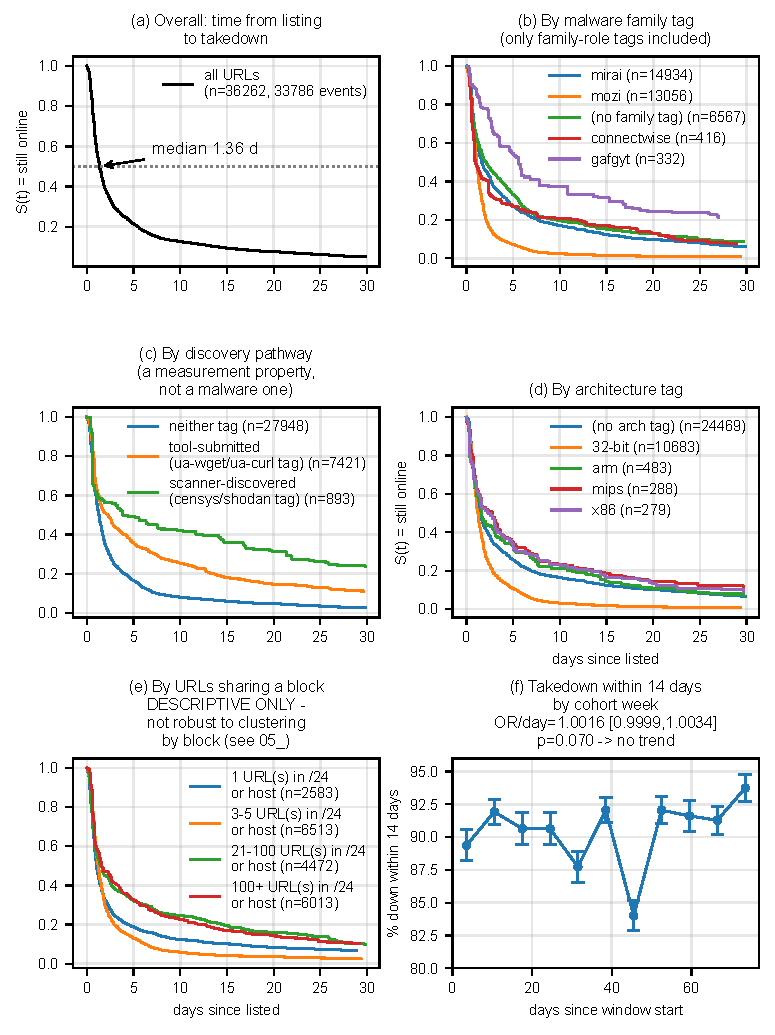
\includegraphics[width=0.86\textwidth]{figures/E0_infra_takedown.pdf}
\caption{Survival of listed malicious infrastructure (E0). Kaplan--Meier survival
over 36{,}262 URLhaus records listed between 2026-06-25 and 2026-09-23 (89 days),
33{,}786 events and 2{,}476 censored entries. Every duration is a lower bound:
\texttt{last\_online} records the last sighting of a URL, not the instant it was
taken down. (a) All URLs. (b) By malware family tag; only family-role tags are
included. (c) By discovery pathway, which is a property of the measurement route
rather than of the malware. (d) By architecture tag. (e) By how many URLs share a
/24 block or a host; this panel is descriptive only and is not robust to
clustering by block. (f) Takedown within 14 days by cohort week, with the fitted
logistic trend OR/day $=1.0016$ $[0.9999, 1.0034]$, $p=0.070$, i.e.\ no trend.
Source: URLhaus; audited result artifact available from the corresponding
author.\label{figS1}}
\end{figure}

\section*{S5. Data, time coverage, licence and ethics supplement}

\subsection*{S5.1 Per-source time coverage}

The three layers do not share a time axis. The AlphaBay full-site archive is
right-censored at a single instant (2017-01-28) and carries no seller identifier,
which is why the social-layer unit of analysis is the listing rather than the
vendor. Agora spans 2014--2015. The Kilos cross-market review panels and the
drug-listing corpus carry no date column at all, so no window can be stated for
them. The Elliptic++ time axis is \textbf{ordinal steps}, not calendar dates;
it can nevertheless be anchored from outside the data, because the steps span
blocks 391,200--487,975 at 2,016 blocks per step, so block 400,000 = 2016-02-25
placed against 144 blocks/day maps the window to approximately 2016-01-01 to
2017-11-03 and puts the July 2017 enforcement wave at steps 41--43. The map is
approximate to $\pm$1 step (roughly two weeks); it is the only calendar anchor
available in the financial layer, and nothing else in the paper depends on it.
The URLhaus and ThreatFox feeds are rolling-retention: an old URL survives in the
dump only while it still resolves, so removal times exist only inside the recent
window.

\subsection*{S5.2 Additional and context sources}

Two further social-layer sources were acquired and probed for the
cross-layer-bridging hypothesis that E3 reports as unmeasurable: the Hansa and
Valhalla dumps (51,553 reviews and 16,511 listings). No reported quantity is
drawn from them. Nine monthly global breach-posture reports (2025-01 through
2025-11, with 05 and 09 absent) are used only as qualitative motivation, because
their per-issue filtering windows drift and the 2025-10 issue's window covers
September; they are not used as evidence.

\subsection*{S5.3 Licence and ethics detail}

We use metadata and public archives only; no raw leaked personal records are
touched; identifiers are hashed. Eight sources are public archives used under
research terms. Two Gwern-curated archives carry no explicit licence and are
treated as research fair use and flagged for the community; the Abuse.ch feeds
are free for research with attribution requested; the Elliptic++ datasets are
public datasets for research use. The nine breach reports' known window defects
are disclosed rather than discovered by a reviewer later. LLM-based tooling was
used in exploratory analysis only, and no reported number depends on
LLM-generated labels, because that pipeline never reached data acquisition. An
early packaging artifact contained a default service credential; it was rotated,
purged from all packaged snapshots, and the incident is disclosed rather than
left discoverable. The rotation and the purge are recorded in the repository's
\texttt{ERRATA.md} and in the project's append-only ledger (\texttt{C-181}), so
that the claim can be checked rather than taken on trust.

\end{document}
